\chapter{PLL (Phase-Locked Loop)}

\section*{Resumen}

En este capítulo se presenta el desarrollo e integración del PLL utilizado para la generación de la señal FMCW. El sistema se basa en el sintetizador de frecuencia ADF4159 y utiliza una placa de evaluación como plataforma para su implementación, complementada con el filtro de lazo diseñado y construido específicamente para esta aplicación. El objetivo principal es integrar los diferentes bloques del sistema y verificar mediante simulación y análisis temporal su capacidad para generar el barrido de frecuencia requerido.

\section{Introducción}

Un \textit{Phase-Locked Loop} (PLL) es un sistema de control realimentado utilizado para sincronizar la fase y, consecuentemente, la frecuencia de una señal de salida con respecto a una señal de referencia. En aplicaciones de síntesis de frecuencia, el PLL permite generar señales de alta frecuencia manteniendo una relación definida con una referencia de frecuencia estable.

En el presente trabajo, el PLL se utiliza como parte del generador de señales FMCW, donde además de sintetizar la frecuencia de salida se requiere realizar un barrido controlado de frecuencia. El sistema debe generar una señal que varíe entre $1{,}55~\mathrm{GHz}$ y $1{,}85~\mathrm{GHz}$, correspondiente a un ancho de banda de $300~\mathrm{MHz}$, con un tiempo de barrido de $0{,}25~\mathrm{ms}$ para las aplicaciones de barridos triangulares y $1~\mathrm{ms}$ para barridos de diente de sierra. Esta condición introduce un requerimiento adicional respecto de una aplicación convencional de síntesis de frecuencia, ya que el PLL debe ser capaz de seguir las variaciones de frecuencia impuestas por la modulación de rampa sin perder el enganche.

Para la implementación se seleccionó el sintetizador ADF4159 de Analog Devices, debido a que incorpora funciones específicas para la generación de rampas de frecuencia y permite configurar los parámetros necesarios para aplicaciones FMCW. El dispositivo se implementa mediante su placa de evaluación, la cual proporciona los elementos necesarios para el funcionamiento del sintetizador y facilita su configuración y caracterización.

La placa de evaluación constituye el núcleo del sistema, incorporando el detector de fase y frecuencia (PFD), la bomba de carga, el divisor de frecuencia y los circuitos auxiliares asociados al sintetizador. A esta plataforma se integra el filtro diseñado en el capítulo anterior, encargado de procesar la corriente proveniente de la bomba de carga y generar la tensión de control aplicada al VCO.

El VCO utilizado en el sistema es el modelo CVCO55BE-1530-2700, cuya frecuencia de operación comprende el intervalo requerido para el barrido. La tensión de control necesaria para recorrer dicho intervalo constituye uno de los principales parámetros considerados durante el diseño del filtro, por lo que la integración entre ambos bloques resulta fundamental para el funcionamiento del PLL.

A diferencia del análisis realizado en el capítulo anterior, donde se estudió el filtro de manera independiente, en este capítulo se considera el comportamiento del sistema completo. Esto permite analizar la interacción entre los distintos bloques y determinar parámetros fundamentales como la frecuencia de cruce, el margen de fase, el ancho de banda efectivo y la capacidad del PLL para seguir la rampa de frecuencia requerida.

\section{Arquitectura del PLL}

El sistema implementado está compuesto principalmente por el sintetizador ADF4159, el filtro de lazo diseñado, el VCO y los elementos de realimentación asociados. Para facilitar el desarrollo experimental, se utiliza la placa de evaluación del ADF4159 como plataforma de integración del sintetizador.

La estructura general del PLL puede describirse mediante los siguientes bloques:

\begin{itemize}
\item Generador de referencia.
\item Detector de fase y frecuencia (PFD).
\item Bomba de carga (\textit{Charge Pump}).
\item Filtro del PLL.
\item Oscilador controlado por tensión (VCO).
\item Divisor de frecuencia de realimentación.
\end{itemize}

El PFD compara la señal de referencia con la señal realimentada proveniente del divisor de frecuencia. A partir de la diferencia de fase entre ambas señales, la bomba de carga genera una corriente que es procesada por el filtro. La tensión resultante se aplica al terminal de control del VCO, modificando su frecuencia de oscilación. Una fracción de la señal de salida del VCO es realimentada mediante el divisor de frecuencia hacia la entrada del PFD, cerrando de esta manera el lazo de control.

\section{Función de transferencia del PLL}
Una vez definidos los distintos bloques que conforman el sintetizador, se procedió a obtener la función de transferencia del PLL.

La configuración utilizada en el ADF4159 establece una frecuencia de referencia de $100~\mathrm{MHz}$ y un divisor de referencia $R=2$. Por lo tanto, la frecuencia aplicada al detector de fase y frecuencia (PFD) resulta:

\begin{equation}
f_{\mathrm{PFD}} = \frac{f_{\mathrm{REF}}}{R} = \frac{100~\mathrm{MHz}}{2} = 50~\mathrm{MHz}.
\end{equation}

El divisor de realimentación se configuró con $N=34$, por lo que la frecuencia de salida correspondiente a la frecuencia central del sistema es:

\begin{equation}
f_{\mathrm{OUT}} = N f_{\mathrm{PFD}} = 34(50~\mathrm{MHz}) = 1{,}7~\mathrm{GHz}.
\end{equation}

De esta manera, los parámetros principales utilizados para el modelado del PLL son:
\begin{equation}
f_{\mathrm{REF}} = 100~\mathrm{MHz},
\qquad
R = 2,
\qquad
f_{\mathrm{PFD}} = 50~\mathrm{MHz},
\qquad
N = 34.
\end{equation}

\subsection*{Ganancia del detector de fase y bomba de carga}
La corriente de la bomba de carga del ADF4159 fue configurada en:
\begin{equation}
I_{\mathrm{CP}} = 2{,}5~\mathrm{mA}.
\end{equation}

Considerando la ganancia del detector de fase y la bomba de carga respecto de la diferencia de fase, se obtiene:

\begin{equation}
K_{\mathrm{PFD}} = \frac{I_{\mathrm{CP}}}{2\pi}.
\end{equation}

Por lo tanto,

\begin{equation}
K_{\mathrm{PFD}} = \frac{2{,}5\times10^{-3}}{2\pi} \approx 3{,}98\times10^{-4}~\mathrm{A/rad}.
\end{equation}

\subsection*{Ganancia del VCO}
Para obtener la ganancia del VCO se utilizaron las mediciones realizadas. El rango de operación considerado comprende una frecuencia de $1{,}55~\mathrm{GHz}$ para una tensión de control de $1{,}19~\mathrm{V}$ y una frecuencia de $1{,}85~\mathrm{GHz}$ para una tensión de control de $3{,}15~\mathrm{V}$.

La sensibilidad del VCO se obtiene mediante:

\begin{equation}
K_{\mathrm{VCO}} = \frac{\Delta f_{\mathrm{VCO}}}{\Delta V_{\mathrm{tune}}}.
\end{equation}

Reemplazando los valores medidos:

\begin{equation}
K_{\mathrm{VCO}} = \frac{1{,}85 - 1{,}55}{3{,}15 - 1{,}19} \approx 0{,}1531~\mathrm{GHz/V} = 153{,}1~\mathrm{MHz/V}.
\end{equation}

Para el análisis de la función de transferencia de fase, la ganancia del VCO debe expresarse en radianes por segundo por voltio. Por lo tanto,

\begin{equation}
K_{\mathrm{VCO,rad}} = 2\pi K_{\mathrm{VCO}}
\end{equation}
y se obtiene:

\begin{equation}
K_{\mathrm{VCO,rad}} = 2\pi(153{,}1\times10^6) \approx 9{,}62\times10^8~\frac{\mathrm{rad/s}}{\mathrm{V}}.
\end{equation}

El VCO puede modelarse, en términos de fase, mediante un integrador:

\begin{equation}
H_{\mathrm{VCO}}(s) = \frac{K_{\mathrm{VCO,rad}}}{s} = \frac{9{,}62\times10^8}{s}.
\end{equation}

\subsection*{Función de transferencia del filtro}
El filtro utilizado en el PLL corresponde a la topología activa inversora desarrollada previamente, la cual presenta los siguientes polos y ceros:
\begin{align}
\omega_z &= 6{,}77\times10^5~\mathrm{rad/s}, \\
\omega_{p2} &= 2{,}59\times10^7~\mathrm{rad/s}, \\
\omega_{p3} &= 6{,}77\times10^6~\mathrm{rad/s}, \\
\omega_{p4} &= 4{,}54\times10^7~\mathrm{rad/s}.
\end{align}

Además, la función de transferencia presenta un polo en el origen. Por lo tanto, su estructura general puede expresarse como:
\begin{equation}
F(s) = K_F \frac{1 + s/\omega_z}{s \left(1 + s/\omega_{p2}\right) \left(1 + s/\omega_{p3}\right) \left(1 + s/\omega_{p4}\right)},
\end{equation}
donde $K_F$ representa la ganancia asociada a la topología activa del filtro.

Esta estructura presenta un polo en el origen, responsable del comportamiento integrador del filtro, y un cero ubicado en aproximadamente $107{,}8~\mathrm{kHz}$, que proporciona adelanto de fase en la región próxima a la frecuencia de cruce.

\subsection*{Divisor de frecuencia}
La señal generada por el VCO es aplicada al divisor de frecuencia del ADF4159. Para la configuración utilizada, el factor de división es:
\begin{equation}
N = 34.
\end{equation}

Por lo tanto, la función de transferencia asociada al divisor es:

\begin{equation}
H_N(s) = \frac{1}{N} = \frac{1}{34}.
\end{equation}

\subsection*{Función de transferencia de lazo abierto}
La función de transferencia de lazo abierto se obtiene mediante el producto de las funciones de transferencia correspondientes a cada uno de los bloques que conforman el lazo:

\begin{equation}
G(s) = K_{\mathrm{PFD}} F(s) \frac{K_{\mathrm{VCO,rad}}}{s} \frac{1}{N}.
\end{equation}

Sustituyendo la expresión obtenida para el filtro:

\begin{equation}
G(s) = \frac{K_{\mathrm{PFD}} K_F K_{\mathrm{VCO,rad}}}{N} \frac{1 + s/\omega_z}{s^2 \left(1 + s/\omega_{p2}\right) \left(1 + s/\omega_{p3}\right) \left(1 + s/\omega_{p4}\right)}.
\end{equation}

Utilizando los valores determinados anteriormente:

\begin{equation}
\frac{K_{\mathrm{PFD}} K_{\mathrm{VCO,rad}}}{N} = \frac{(3{,}98\times10^{-4})(9{,}62\times10^8)}{34} \approx 1{,}13\times10^4.
\end{equation}

Para determinar la capacitancia total equivalente del filtro de lazo ($A_0$), se impone la condición de que la magnitud de la función de transferencia de lazo abierto sea unitaria ($0~\mathrm{dB}$) en la frecuencia de cruce $\omega_c$. A partir de esto, se obtiene la siguiente expresión:

\begin{equation}
A_0 = \frac{K_{\mathrm{PFD}} K_{\mathrm{VCO,rad}}}{N \omega_c^2} \sqrt{\frac{1 + (\omega_c T_2)^2}{\left[1 + (\omega_c T_1)^2\right] \left[1 + (\omega_c T_3)^2\right] \left[1 + (\omega_c T_4)^2\right]}}.
\end{equation}

La frecuencia de cruce en radianes por segundo se obtiene a partir del ancho de banda simulado:

\begin{equation}
\omega_c = 2\pi (293\times10^3) \approx 1{,}841\times10^6~\mathrm{rad/s}.
\end{equation}

Para simplificar el cálculo, se evalúan de forma independiente las relaciones al cuadrado entre la frecuencia de cruce y las frecuencias de corte de cada polo y cero $(\omega_c / \omega_{\mathrm{corte}})^2$:

\begin{align}
    (\omega_c T_2)^2 &= \left(\frac{1{,}841\times10^6}{6{,}77\times10^5}\right)^2 \approx 7{,}395, \\
    (\omega_c T_1)^2 &= \left(\frac{1{,}841\times10^6}{2{,}59\times10^7}\right)^2 \approx 0{,}005, \\
    (\omega_c T_3)^2 &= \left(\frac{1{,}841\times10^6}{6{,}77\times10^6}\right)^2 \approx 0{,}074, \\
    (\omega_c T_4)^2 &= \left(\frac{1{,}841\times10^6}{4{,}54\times10^7}\right)^2 \approx 0{,}0016.
\end{align}

Sustituyendo estos términos y la constante de ganancia de lazo deducida previamente en la ecuación de $A_0$:

\begin{equation}
A_0 = \frac{1{,}13\times10^4}{(1{,}841\times10^6)^2} \sqrt{\frac{1 + 7{,}395}{(1 + 0{,}005) (1 + 0{,}074) (1 + 0{,}0016)}}.
\end{equation}

Resolviendo las operaciones en el numerador y denominador:

\begin{equation}
A_0 = \left( \frac{1{,}13\times10^4}{3{,}389\times10^{12}} \right) \sqrt{\frac{8{,}395}{1{,}081}}.
\end{equation}

\begin{equation}
A_0 = (3{,}334\times10^{-9}) (2{,}786) \approx 9{,}28\times10^{-9}~\mathrm{F}.
\end{equation}

El valor obtenido, $A_0 = 9{,}28~\mathrm{nF}$, representa la capacitancia total del filtro activo. Con este parámetro, la constante multiplicativa del filtro resulta $K_F = 1/A_0 \approx 1{,}07\times10^8$.

Sustituyendo la constante $K_F$ deducida y los parámetros del sistema en la función de lazo abierto:

\begin{equation}
G(s) = 1{,}21\times10^{12} \frac{1 + s/(6{,}77\times10^5)}{s^2 \left(1 + s/(2{,}59\times10^7)\right) \left(1 + s/(6{,}77\times10^6)\right) \left(1 + s/(4{,}54\times10^7)\right)}.
\end{equation}

Con el objetivo de verificar el comportamiento de la función de transferencia de lazo abierto obtenida analíticamente, se realizó su evaluación mediante MATLAB. A partir de la expresión anterior se calculó la respuesta en frecuencia del sistema, obteniéndose el diagrama de Bode mostrado en la Figura~\ref{fig:bode_lazo_abierto}.

\begin{figure}[H]
    \centering
    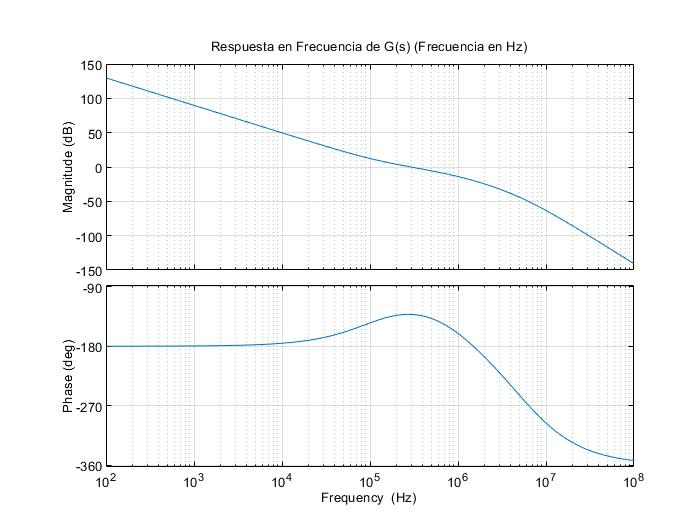
\includegraphics[width=0.75\textwidth]{imagenes/bode_lazo_abierto_matlab.jpg}
    \caption{Respuesta en frecuencia de la función de transferencia de lazo abierto obtenida mediante MATLAB. (Fuente: propia).}
    \label{fig:bode_lazo_abierto}
\end{figure}

\subsection*{Función de transferencia de lazo cerrado}
La función de transferencia a lazo cerrado $CL(s)$ relaciona la fase de salida del VCO con la fase de la señal de referencia. Se define como:

\begin{equation}
CL(s) = \frac{G_{\mathrm{fwd}}(s)}{1 + G_{\mathrm{fwd}}(s) \cdot H}
\end{equation}

Donde $H = 1/N$ es el factor de realimentación y $G_{\mathrm{fwd}}(s)$ es la ganancia de la trayectoria directa. Dado que la función de lazo abierto $G(s)$ deducida previamente ya incorpora el divisor $N$, se cumple que $G_{\mathrm{fwd}}(s) = N \cdot G(s)$. Sustituyendo, la ecuación de lazo cerrado se expresa en función de la ganancia de lazo abierto como:

\begin{equation}
CL(s) = \frac{N \cdot G(s)}{1 + G(s)}.
\end{equation}

Para evaluar esta expresión, se definen el numerador $\text{Num}(s)$ y el denominador $\text{Den}(s)$ de la función de lazo abierto $G(s)$:

\begin{align}
\text{Num}(s) &= 1{,}21\times10^{12} \left(1 + \frac{s}{6{,}77\times10^5}\right), \\
\text{Den}(s) &= s^2 \left(1 + \frac{s}{2{,}59\times10^7}\right) \left(1 + \frac{s}{6{,}77\times10^6}\right) \left(1 + \frac{s}{4{,}54\times10^7}\right).
\end{align}

Sustituyendo estos términos, la función de transferencia total a lazo cerrado resulta:

\begin{equation}
CL(s) = 34 \cdot \frac{\text{Num}(s)}{\text{Den}(s) + \text{Num}(s)},
\end{equation}

\begin{equation}
CL(s) = \frac{4{,}11\times10^{13} \left(1 + \dfrac{s}{6{,}77\times10^5}\right)}{s^2 \left(1+\dfrac{s}{2{,}59\times10^7}\right) \left(1+\dfrac{s}{6{,}77\times10^6}\right) \left(1+\dfrac{s}{4{,}54\times10^7}\right) + 1{,}21\times10^{12} \left(1 + \dfrac{s}{6{,}77\times10^5}\right)}.
\end{equation}

El polinomio característico resultante en el denominador es de quinto orden. Las raíces de este polinomio corresponden a los polos de lazo cerrado del sistema, los cuales dictaminan la estabilidad, el tiempo de bloqueo (\textit{lock time}) y la respuesta transitoria del sintetizador.

Para verificar el comportamiento del sistema a lazo cerrado, se evaluó en MATLAB la función de transferencia $CL(s)$ obtenida analíticamente. A partir de la expresión anterior se calculó la respuesta en frecuencia del sistema, obteniéndose el diagrama de Bode mostrado en la Figura~\ref{fig:respuesta_lazo_cerrado}.

\begin{figure}[H]
    \centering
    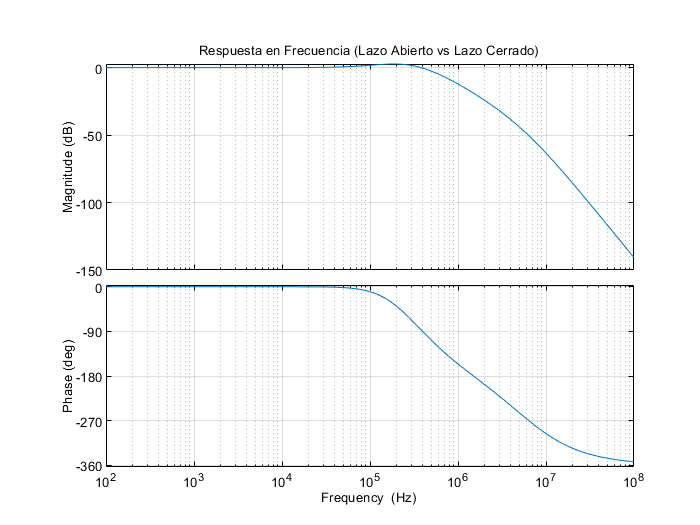
\includegraphics[width=0.75\textwidth]{imagenes/bode_lazo_cerrado_matlab.png}
    \caption{Respuesta en frecuencia de la función de transferencia de lazo cerrado obtenida mediante MATLAB. (Fuente: propia).}
    \label{fig:respuesta_lazo_cerrado}
\end{figure}

\section{Simulación del PLL}

Una vez finalizado el diseño del filtro de lazo y obtenidas las funciones de transferencia del sistema, se realizó la simulación completa del PLL mediante la herramienta \textit{ADIsimPLL} de Analog Devices. El objetivo de esta simulación es verificar el comportamiento del sistema de la Figura~\ref{fig:adisimpll_esquema} a partir de los parámetros obtenidos durante el diseño y comprobar que el PLL cumple con los requerimientos de ancho de banda, estabilidad y velocidad de respuesta establecidos.

\begin{figure}[H]
    \centering
    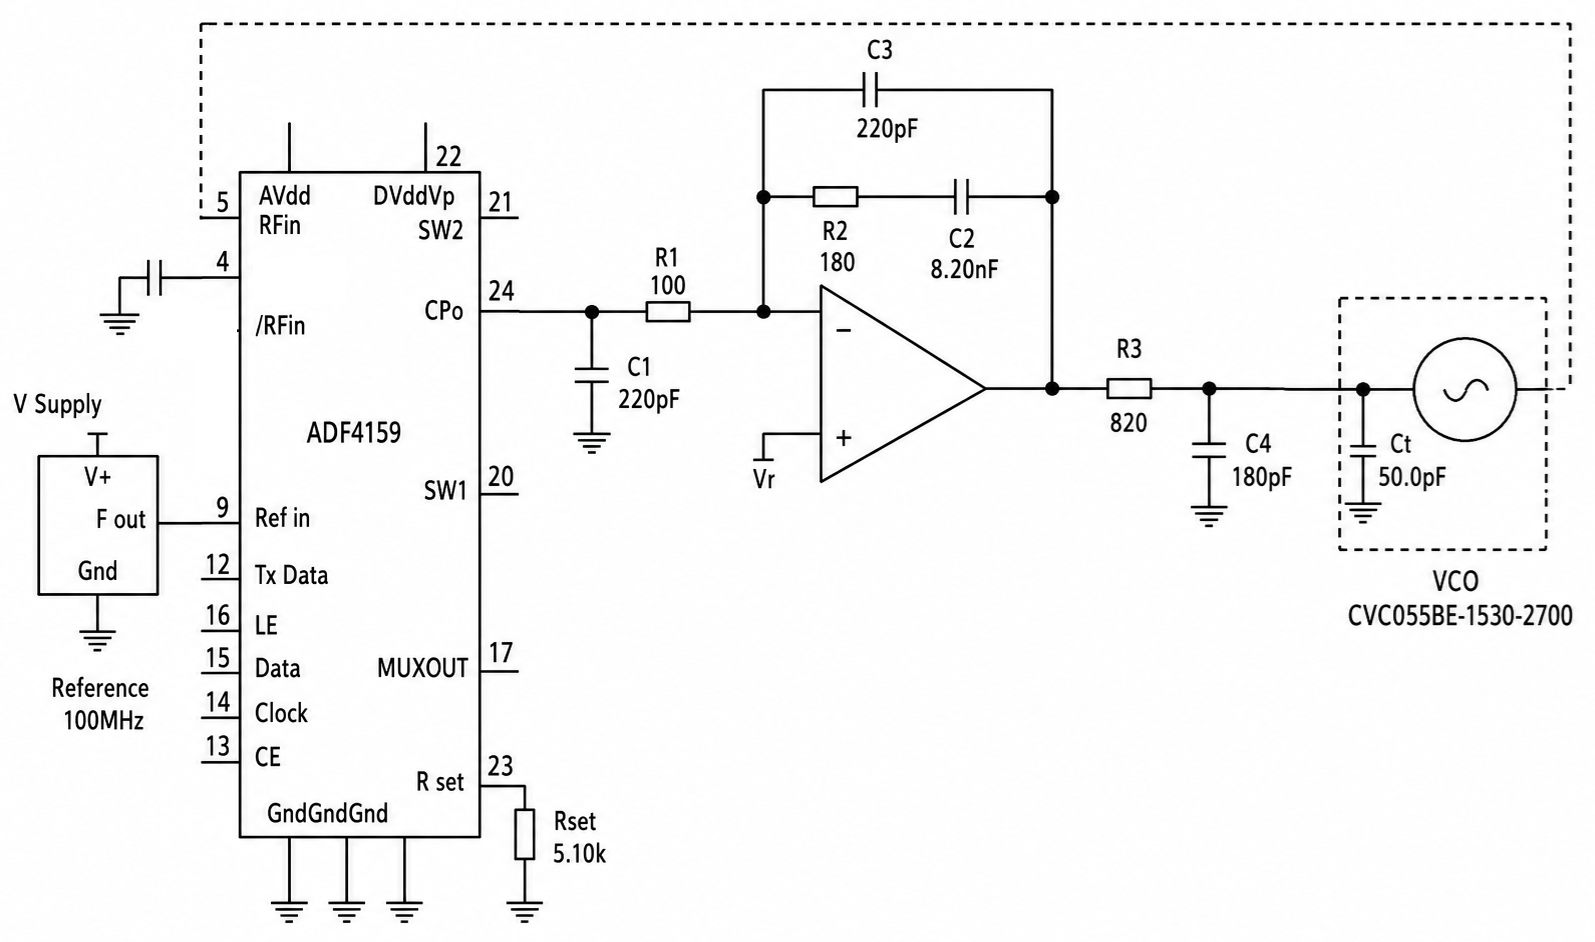
\includegraphics[width=0.8\linewidth]{imagenes/esquemapll_adisim.png}
    \caption{Esquema analizado en ADIsimPLL. (Fuente: propia).}
    \label{fig:adisimpll_esquema}
\end{figure}

Se evaluó la respuesta de la función de transferencia de lazo abierto, con el objetivo de verificar la frecuencia de cruce y los márgenes de estabilidad obtenidos para el diseño. El resultado de esta simulación se presenta en la Figura~\ref{fig:adisimpll_lazo_abierto}.

\begin{figure}[H]
\centering
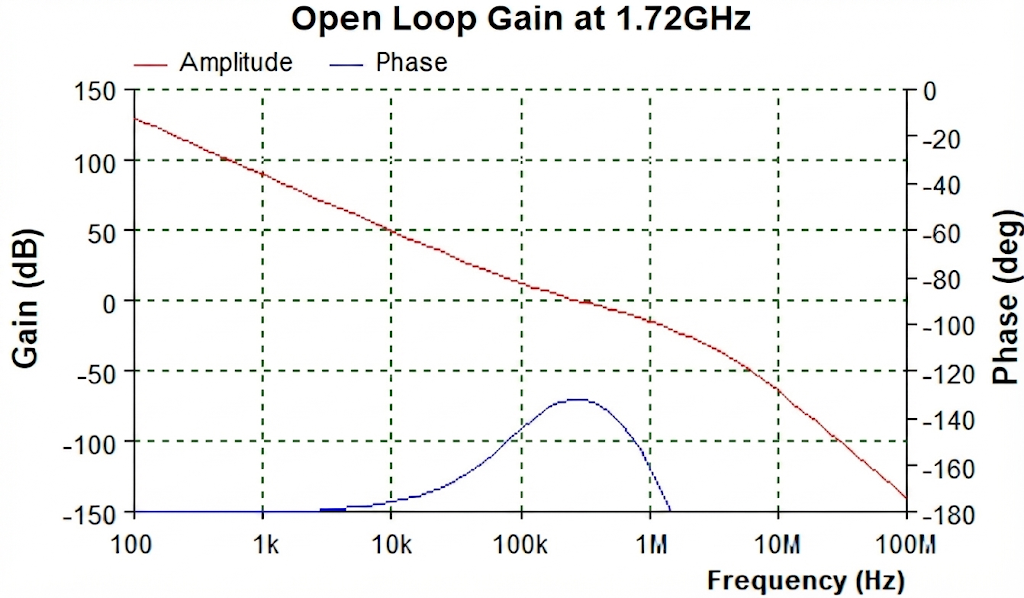
\includegraphics[width=0.75\textwidth]{imagenes/adisimpll_lazo_abierto.png}
\caption{Respuesta de la función de transferencia de lazo abierto obtenida mediante ADIsimPLL. (Fuente: propia).}
\label{fig:adisimpll_lazo_abierto}
\end{figure}

A continuación, se analizó la respuesta del sistema a lazo cerrado. Esta simulación permite verificar el comportamiento global del PLL y determinar el ancho de banda efectivo del sistema. La respuesta obtenida mediante ADIsimPLL se muestra en la Figura~\ref{fig:adisimpll_lazo_cerrado}.

\begin{figure}[H]
\centering
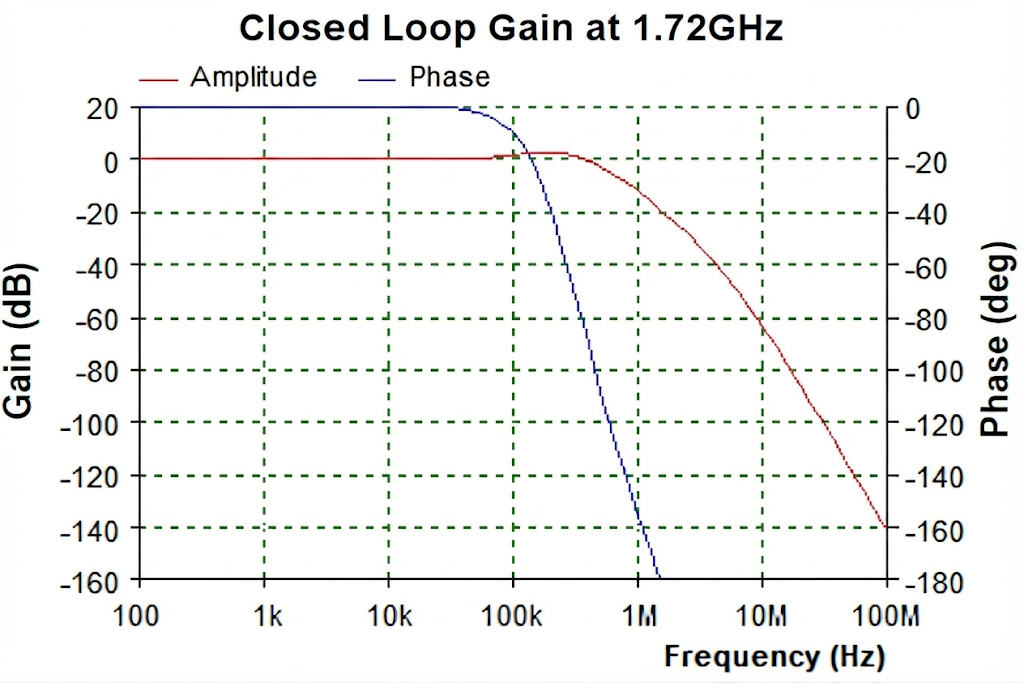
\includegraphics[width=0.75\textwidth]{imagenes/adisimpll_lazo_cerrado.png}
\caption{Respuesta de la función de transferencia a lazo cerrado obtenida mediante ADIsimPLL. (Fuente: propia).}
\label{fig:adisimpll_lazo_cerrado}
\end{figure}

Finalmente, se evaluó la respuesta transitoria del PLL ante un cambio de frecuencia de referencia. Para ello, se configuró un salto desde $1{,}55~\mathrm{GHz}$ hasta $1{,}85~\mathrm{GHz}$, permitiendo analizar directamente la capacidad del sintetizador para alcanzar la nueva frecuencia de operación. Esta prueba resulta particularmente importante debido a que permite determinar el tiempo de establecimiento (\textit{lock time}) del PLL y verificar que la dinámica del sistema sea compatible con los requerimientos de velocidad definidos para la aplicación.

La respuesta temporal obtenida mediante ADIsimPLL se presenta en la Figura~\ref{fig:adisimpll_lock_time}, donde se observa la transición entre ambas frecuencias y el posterior establecimiento de la señal de salida.

\begin{figure}[H]
\centering
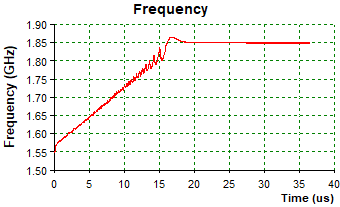
\includegraphics[width=0.65\textwidth]{imagenes/adisimpll_lock_time.png}
\caption{Respuesta transitoria del PLL ante un salto de frecuencia de $1{,}55~\mathrm{GHz}$ a $1{,}85~\mathrm{GHz}$ obtenida mediante ADIsimPLL. (Fuente: propia).}
\label{fig:adisimpll_lock_time}
\end{figure}

A partir de esta última simulación se determina el tiempo de establecimiento del PLL, definido como el intervalo transcurrido desde la aplicación del cambio de frecuencia hasta que la salida permanece dentro del margen de error especificado alrededor de la frecuencia final. El valor obtenido permite evaluar la capacidad del sintetizador para realizar cambios rápidos de frecuencia y constituye un parámetro fundamental para la validación final del diseño.

\section{Desarrollo del PLL}

Para el desarrollo del PLL se seleccionó el sintetizador de frecuencia ADF4159 de Analog Devices. La elección de este dispositivo se debe principalmente a la flexibilidad que ofrece para adaptar los diferentes bloques del PLL a los requerimientos específicos de la aplicación. A diferencia de otras soluciones integradas, el ADF4159 no incorpora un VCO ni un filtro de lazo internos.

Esta característica resulta particularmente conveniente para el presente proyecto, ya que permite utilizar un VCO externo y modificar sus características de sintonía de acuerdo con la frecuencia de operación requerida. El dispositivo permite trabajar con VCOs externos dentro de un amplio rango de frecuencias, aproximadamente entre $0{,}5~\mathrm{GHz}$ y $13~\mathrm{GHz}$, proporcionando la flexibilidad necesaria para seleccionar el oscilador en función de la aplicación. Del mismo modo, al no integrar el filtro de lazo, es posible diseñar su topología y seleccionar sus componentes de acuerdo con los requerimientos de ancho de banda, estabilidad y velocidad de respuesta del sistema.

Otra característica relevante del ADF4159 es la modulación en frecuencia, lo que permite su uso como generador de rampa interno. Esta funcionalidad resulta especialmente útil para la aplicación desarrollada, ya que permite generar barridos de frecuencia de forma programable desde el propio sintetizador, simplificando considerablemente el control digital.

Para el desarrollo y simulación del PLL se utilizó la placa de evaluación EV-ADF4159EB3Z, correspondiente al ADF4159. Esta placa se tomó como plataforma para la configuración del sintetizador y para la integración de los distintos bloques que conforman el sistema. La Figura~\ref{fig:ev_adf4159_pll} muestra la placa de evaluación utilizada como referencia. La imagen y los valores correspondientes a la configuración del dispositivo fueron obtenidos de la documentación proporcionada por el fabricante~\cite{ADF4159EB3Z}.

\begin{figure}[H]
\centering
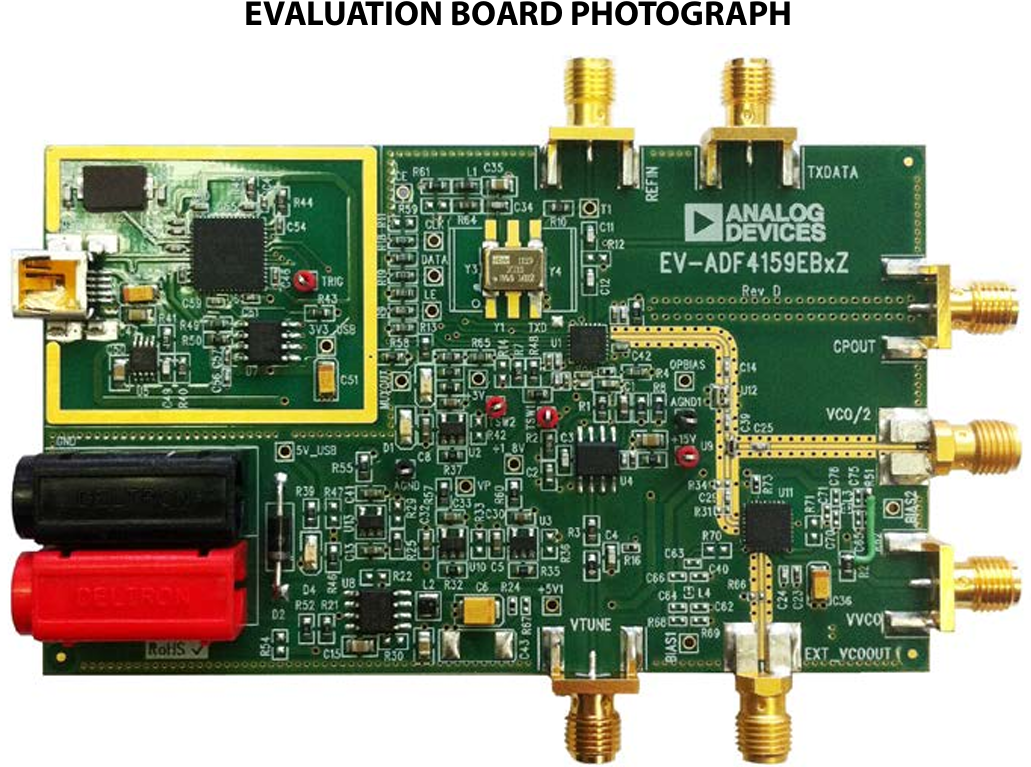
\includegraphics[width=0.85\textwidth]{imagenes/EV-ADF4159EB3Z.png}
\caption{Placa de evaluación EV-ADF4159EB3Z utilizada como referencia para el desarrollo del PLL. (Fuente: \cite{ADF4159EB3Z}).}
\label{fig:ev_adf4159_pll}
\end{figure}

El filtro implementado, presentado en el capítulo anterior, constituye la interfaz entre la bomba de carga del ADF4159 y el VCO. Su función es convertir la corriente generada por la bomba de carga en una tensión de control adecuada, al mismo tiempo que establece la dinámica del lazo mediante la incorporación de los polos y ceros definidos durante el proceso de diseño.

La salida del filtro se conecta al terminal de sintonía del VCO CVCO55BE-1530-2700. El rango de tensión requerido para generar el barrido de frecuencia se encuentra comprendido entre $1{,}19~\mathrm{V}$ y $3{,}15~\mathrm{V}$. Por lo tanto, la correcta integración entre el filtro y el VCO resulta fundamental para garantizar que el PLL pueda recorrer la totalidad del intervalo de frecuencia especificado.

La señal generada por el VCO constituye la salida del sistema y, simultáneamente, la señal de realimentación del PLL.

\section{Medición}

Una vez finalizada la implementación del PLL, se realizó la medición experimental de la respuesta temporal de la tensión de control del VCO con el objetivo de verificar el comportamiento del sistema frente a un cambio de frecuencia. Para esta prueba se configuró un salto de frecuencia desde $1{,}55~\mathrm{GHz}$ hasta $1{,}85~\mathrm{GHz}$, correspondiente a una variación de $300~\mathrm{MHz}$.

De esta manera, el resultado medido puede compararse con la respuesta obtenida mediante la simulación en ADIsimPLL, permitiendo evaluar la correspondencia entre el comportamiento teórico y el circuito implementado.

La respuesta temporal medida durante el salto de frecuencia se presenta en la Figura~\ref{fig:medicion_lock_time}. En la gráfica se observa la transición desde $1{,}55~\mathrm{GHz}$ hasta $1{,}85~\mathrm{GHz}$ y el posterior establecimiento de la frecuencia de salida.

\begin{figure}[H]
\centering
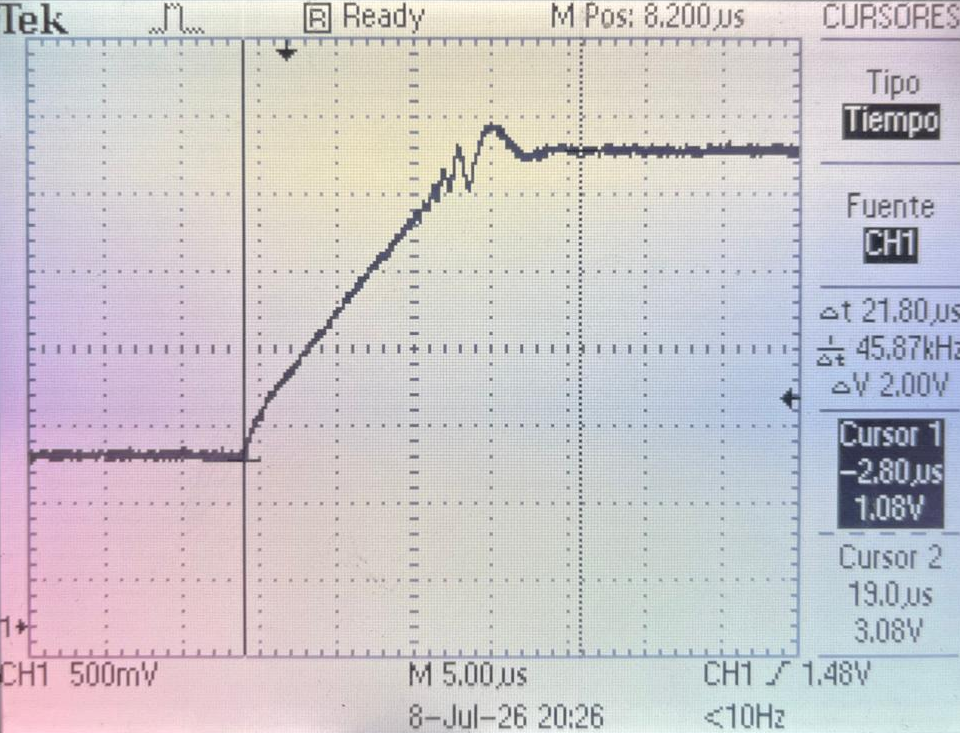
\includegraphics[width=0.55\textwidth]{imagenes/medicion_1550_1850.png}
\caption{Respuesta temporal de la tensión de control medida del PLL ante un salto de frecuencia de $1{,}55~\mathrm{GHz}$ a $1{,}85~\mathrm{GHz}$. (Fuente: propia).}
\label{fig:medicion_lock_time}
\end{figure}

A partir de la respuesta obtenida se determinó experimentalmente el tiempo de establecimiento del PLL en alrededor de $19~\mu\mathrm{s}$, con un tiempo pico de $16{,}2~\mu\mathrm{s}$. Este valor constituye uno de los principales parámetros de validación del diseño, ya que permite comprobar que la dinámica del sistema implementado cumple con los requerimientos establecidos para el barrido de frecuencia, obteniéndose valores muy cercanos a los simulados en ADIsimPLL.